\iffalse%-o-o-o- oude inleiding
Wie had in 1950 gedacht dat we zeventig jaar later computers zouden gebruiken om elkaar kattenfilmpjes toe te sturen? Voorspellen is moeilijk, zeker als het de toekomst betreft. \hrefqr[-2cm]{https://historiek.net/spierballen-nodig-voor-harde-schijf-van-5mb/64614/}{Deze harde schijf} van IBM bevatte net zoveel informatie als een fotootje dat je maakt met je telefoon. Het succes van opkomende technologie is moeilijk te voorspellen.

Klassieke computers worden kleiner en sneller, maar dat is niet het onderwerp van deze module. In deze module maken we kennis met een nieuwe technologie. We zullen ontdekken dat een quantum computer dingen kan die een gewone computer niet kan. De resultaten die met quantum computing behaald zouden \textit{kunnen} worden (we zijn voorzichtig) zijn potentieel van strategisch belang. Tech-giganten als Google, IBM, Alibaba en Amazon investeren nu al miljarden in deze technologie, net als nationale overheden. In Nederland is er de Quantum Delta NL~\cite{qdnl2021}, Europa heeft het European Quantum Flagship~\cite{eqf2017} en ook de VS hebben een strategische agenda gepubliceerd~\cite{usgov2020}. 
In Nederland wordt er aan dit onderwerp op verschillende universiteiten en bedrijven onderzoek gedaan.

Luister eens naar een kort stukje (1:00'30"-1:03'40") uit een lezing van professor  \hrefqr[-2cm]{https://video.leidenuniv.nl/media/t/1_yiuv259f/187033283}{Carlo Beenakker} (Universiteit Leiden). Daarin geeft hij zijn persoonlijke visie.


\section{Ontdekkingen}
De quantum computer is een product van de quantumfysica en de informatiekunde. De quantummechanica is ontstaan uit een noodgreep van Max Planck die rond 1900 het een probleem oploste dat bekend staat als de UV-catastrofe. Hij kon het stralingsgedrag van zwarte lichamen verklaren door een hulpconstante in te voeren (h voor hilfe, later de constante van Planck genoemd). 

In het golf-deeltjes debat dat al speelde sinds Huygens en Newton toonde Einstein~\cite{einstein1905photoelectric} in 1905 in navolging van Planck aan dat licht uit deeltjes (fotonen) bestaat. De Broglie toonde wat later aan dat deeltjes zich als golf konden gedragen. In 1926 formuleerden Erwin Schr\"odinger en Werner Heisenberg de wiskunde van de quantummechanica zoals wij die nu ook nog gebruiken.

%\marginpar{\vspace{2cm}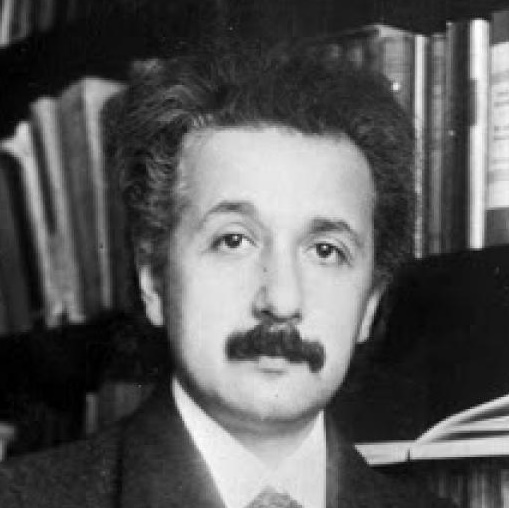
\includegraphics[width=0.95\marginparwidth]{./img/einstein1905.jpg} Einstein: licht bestaat uit energiepaketjes: fotonen}

%\marginpar{\vspace{-2.8cm}\includegraphics[width=0.95\marginparwidth]{./img/debroglie.jpg} DeBroglie: Deeltjes gedragen zich als golven}

Rond 1946 speelden Alan Turing en John von Neumann een belangrijke rol in de ontwikkeling van de informatietheorie. We gaan daar in deze module niet diep op in, maar we constateren dat de computers die wij nu gebruiken nog steeds gebaseerd zijn op het \hrefqr{https://en.wikipedia.org/wiki/Von_Neumann_architecture} {ontwerp} van von Neumann uit 1945.  

In 1982 hield Richard Feynman~\cite{feynman1982simulating} een lezing waarin hij stelde dat een klassieke computer ontoereikend was om quantumsystemen effici\"ent te beschrijven. Een quantum computer zou dat misschien wel kunnen. Kort daarna werden de eerste quantumalgoritmen gepubliceerd. De ontwikkeling van de hardware moest toen nog beginnen.
\medskip
\begin{antwoord}
1998, NMR systeem
\end{antwoord}
\begin{opdracht}\label{opd:tijdlijn}
Wikipedia geeft de geschiedenis van quantum computing in een \hrefqr[-0.5cm]{https://en.wikipedia.org/wiki/Timeline_of_quantum_computing_and_communication}{tijdlijn} weer. 
Wanneer werd de eerste berekening op een quantum computer uitgevoerd? Welke technologie gebruiken zij?
\end{opdracht}
Bijna honderd jaar na de eerste stappen in de quantumwereld start een nieuwe quantumtechnologie: quantum computing. 
\fi%-o-o-o-o

\nogdoen{hieronder opgeschoond 2e draft 20210070}
\iffalse
%\begin{figure}[ht]
\includemovie[
 poster,
 text={\small(click to load singlephotondoubleslit.mp4)}
]{12cm}{4cm}{./img/singlephotondoubleslit.mp4}
%\end{figure}
\fi

\tagged{eruit}{%\iffalse%-----
Met zijn vele tegenintu\"itieve verschijnselen is de quantumwereld een vreemde wereld. In dit hoofdstuk maak je kennis met die vreemde wereld. Daarbij helpt het om de experimenten zelf te doen. In dit hoofdstuk houden we de lijn van de geschiedenis aan. Dat betekent dat je kennis maakt met quantumverschijnselen op een wijze dat je ook inziet hoe de quantumtheorie in de tijd tot stand is gekomen. 
Een sleutelrol is weggelegd voor het licht. Quantummechanica is begonnen met een probleem over elektromagnetische straling waarvan licht deel uitmaakt. Een jongen van \num{25}~jaar ontstak de lont die de gevestigde natuurkunde zou opblazen. Maar om dit alles te kunnen begrijpen is het nodig terug te gaan naar de $17^e$ eeuw. Dat was de tijd van Newton en Huygens. 

\section{Golven of deeltjes?}
De beide geleerden waren het volledig oneens over de aard van het licht. Isaac Newton (1643-1727) geloofde dat licht bestond uit deeltjes. Licht plant zich rechtlijnig voort.

\begin{experiment}{}[blue]
Twee geluidsbron met een toon van ongeveer \SI{1}{\kilo\hertz}. Doe een vinger in je oor en ga met je hoofd langzaam heen en weer. Je zult op sommige plekken extra hard geluid, en op sommige plekken nagenoeg stilte ervaren. De stille plekken noemen we knopen, de extra luide plekken heten buiken. Merk op, deze plekken bewegen niet met de golf mee, ze staan op vaste plekken in de ruimte. Dit verschijnsel noemen we interferentie.

Zoek de voortplantingssnelheid van geluid op.
\end{experiment}


\marginpar{\vspace{0cm}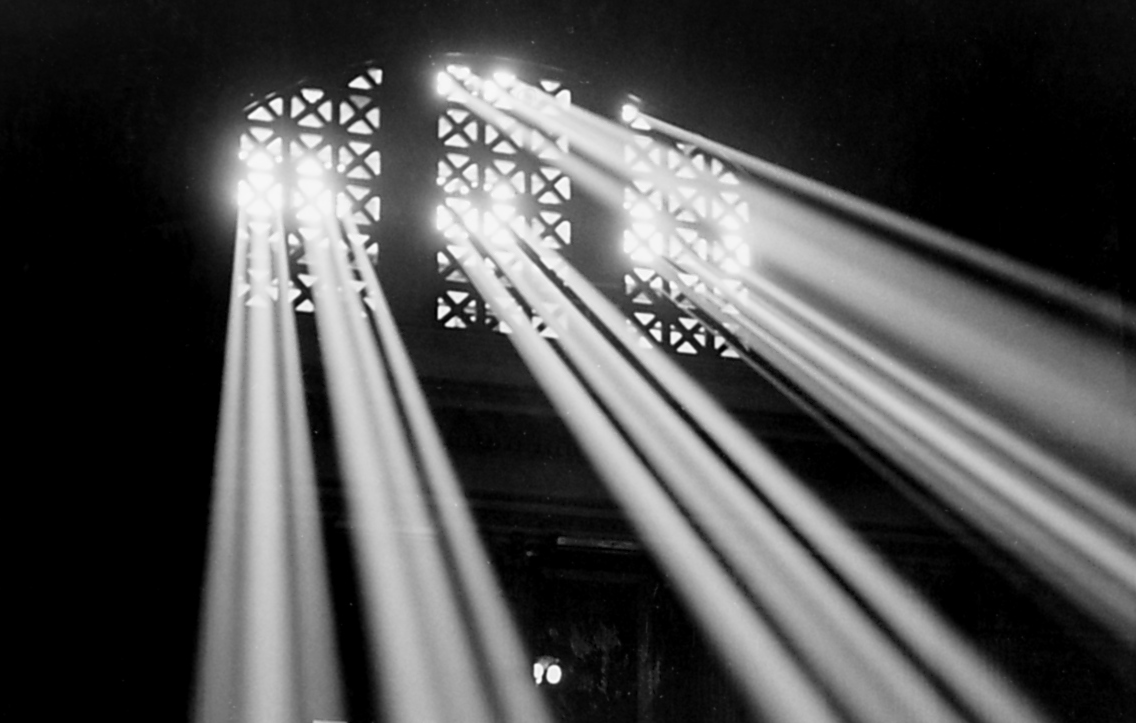
\includegraphics[width=0.95\marginparwidth]{./img/stoffigeruimte.png}
 \captionof{figure}{In een stoffige ruimte worden lichtstralen zichtbaar.
Duidelijk is te zien dat licht zich rechtlijnig voortplant. 
Tegelijkertijd: Je ziet die bundels. Dat kan alleen als niet alle licht recht is doorgegaan. Er ging ook licht naar de cameralens!
 \label {fig:stoffigeruimte}}}

\begin{center}
\leavevmode
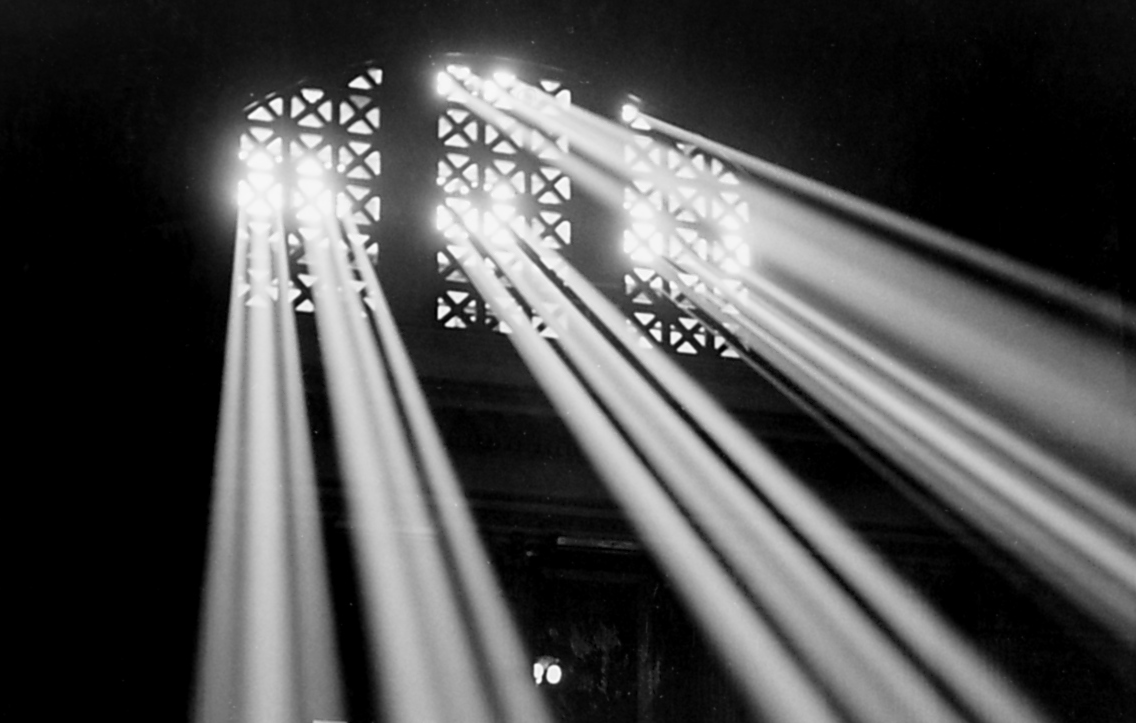
\includegraphics[width=0.5\textwidth]{./img/stoffigeruimte.png}
 \captionof{figure}{In een stoffige ruimte worden lichtstralen zichtbaar.
Duidelijk is te zien dat licht zich rechtlijnig voortplant. 
Tegelijkertijd: Je ziet die bundels. Dat kan alleen als niet alle licht recht is doorgegaan. Er ging ook licht naar de cameralens!
\label {fig:stoffigeruimte2}}
\end{center}

Als licht een golfverschijnsel was geweest, zo meende Newton, had het net als watergolven en geluidsgolven, buiging en interferentie moeten vertonen. Geluiden in een kamer zijn ook op de gang te horen als de deur van de kamer open staat. Maar het licht vanuit de kamer dat in de gang komt wordt scherp begrensd door de schaduw. Licht plant zich rechtlijnig voort. 

Christiaan Huygens (1629-1695) was er van overtuigd dat licht een golfverschijnsel was. Om duidelijk te maken hoe licht zich voortplant maakte hij gebruik van een veronderstelling die bekend geworden is als het principe van Huygens. Dat principe luidt: elk punt dat getroffen wordt door een golf wordt zelf een puntvormige golfbron. Om dit principe toe te lichten dient figuur~\ref{fig:kaarsgolven} die in zijn \textit{"Trait\'e de la lumi\`ere"} is te vinden.


\begin{center}
\leavevmode
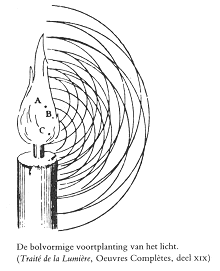
\includegraphics[width=0.5\textwidth]{./img/kaarsgolven.png}
\captionof{figure}{Voortplanting van het licht
De punten A, B en C zijn drie willekeurige punten die door licht worden getroffen en daarmee zelf als puntvormige golfbron gaan functioneren. 
\label {fig:kaarsgolven}
}
\end{center}

In zijn \textit{"Trait\'e de la lumi\`ere"} introduceert Huygens een hulphypothese waarmee hij alle golfverschijnselen te lijf gaat. Deze hulphypothese, bekend geworden als het principe van Huygens, houdt in dat elk punt dat getroffen wordt door lichtgolven zelf gaat functioneren als een puntvormige golfbron. Vanuit de punten A, B en C komen dus bolvormige golven. Getekend zijn de golffronten.
Om te weten wat de lichtsterkte is in een punt P gelegen ver van de kaars af moeten de bijdragen van alle golven worden opgeteld ofwel gesuperponeerd. De techniek om dat voor heel veel golven te doen was nog onbekend in de zeventiende eeuw. 
Heel belangrijk in de geschiedenis van de lichttheorie is de ontdekking geweest van dubbelbreking. Zowel Newton als Huygens waren ervan overtuigd dat als ze een verklaring voor dit verschijnsel zouden kunnen vieren, hun theorie zou zegevieren. 

\section{Dubbelbreking in IJslandspaat}
Erasmus Bartholinus was een tijdgenoot van Newton en Huygens. Deze Deense wiskundige ontdekte in 1669 dat Ijslands Spaat (een zeldzaam doorzichtig calcietkristal) ($\mathrm{CaCO_3}$) dubbelbreking vertoonde. Zie figuur~\ref{fig:ijslandspaat}.


\begin{center}
\leavevmode
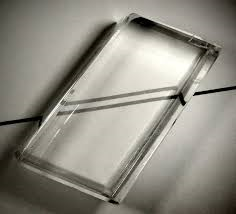
\includegraphics[width=0.5\textwidth]{./img/ijslandspaat.png}
\captionof{figure}{Dubbelbreking door IJslands Spaat (een calcietkristal (CaCO3 )). 
Het licht doorloopt in het kristal niet \'e\'en lichtweg maar twee.
 \label {fig:ijslandspaat}
}
\end{center}

Licht volgt in het kristal twee wegen. Newton probeerde dat te verklaren door aan te nemen dat zijn lichtdeeltjes bepaalde vormen zouden hebben. Huygens probeerde iets met interferentie. Beide geleerden slaagden er uiteindelijk niet in om een sluitende verklaring te geven. Vanwege het grote gezag dat Newton ook op het continent genoot werd zijn deeltjesopvatting de standaard. Pas in de negentiende eeuw kantelde het beeld.

\section{Rond 1800: nieuwe idee\"en}
In het begin van de negentiende eeuw nam een jonge Engelsman, Thomas Young (1773-1829) de handschoen op. Hij toonde als eerste op overtuigende wijze de buigingsverschijnselen aan die er op wijzen dat licht een golfverschijnsel is. Om zijn experiment te kunnen begrijpen is het goed om eerst kennis te maken met interferentieverschijnselen bij geluid.

\section{Experiment Interferentie van geluid}
Geluidsgolven uit twee speakers kunnen elkaar versterken of juist uitdoven. Dit hangt af van de positie van de waarnemer. Om het verschijnsel te onderzoeken maken we gebruik van een toongenerator die een constante toon van ongeveer \SI{1}{\kilo\Herz} voortbrengt. Dit is de frequentie waarop het menselijk oor het gevoeligst is. De speakers zijn aangesloten op de toongenerator.
Bekijk de afbeelding van figuur~\ref{fig:tweebronnen}.



\begin{center}
\leavevmode
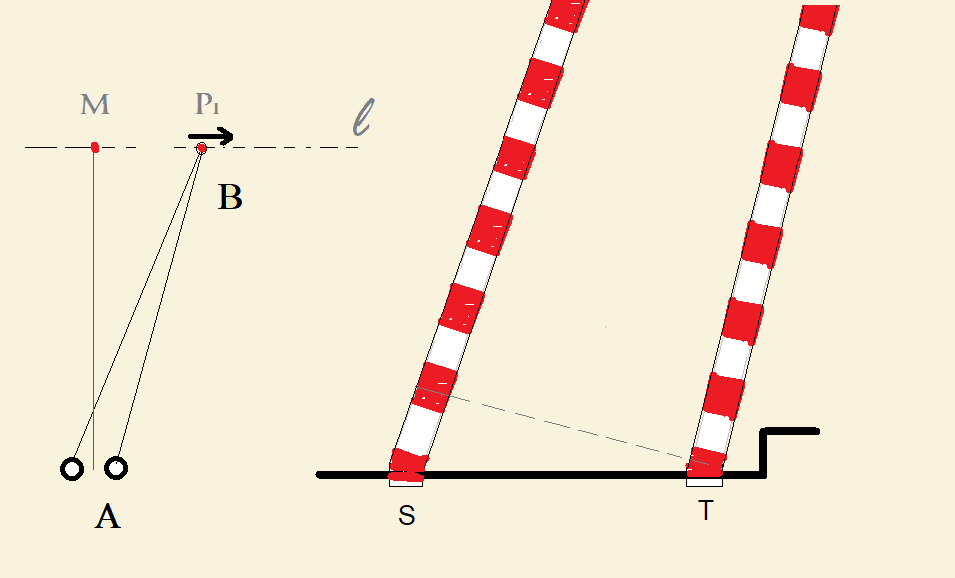
\includegraphics[width=0.5\textwidth]{./img/tweebronnen.png}
\captionof{figure}{Op de lijn $l$ zijn plaatsen te vinden waar het geluid van de twee speakers in $A$ en $B$ heel goed of juist slecht is te horen. Dit wordt veroorzaakt door interferentie. \label {fig:tweebronnen}
}
\end{center}

Een waarnemer die langs de lijn $l$ beweegt hoort afwisselend hard en zacht geluid. In M hoort de waarnemer hard geluid omdat het geluid uit de twee speakers naar M toe een even lange weg moet afleggen. Maar voor elk ander punt op de lijn $l$ is dat niet zo. Er is een weglengteverschil. Het verschijnsel is te simuleren met behulp van Rowili. Dat is de tape die wel wordt gebruikt om een stuk terrein af te bakenen. De rode banden stellen bijvoorbeeld golfbergen voor en de witte banden stellen dan de dalen voor. In de tekening stellen de twee stroken Rowili het geluid voor dat uit de boxen S en T komt. Vanaf het stippellijntje is de afstand tot de waarnemer voor beide stroken gelijk. Bij de waarnemer komen dus altijd ofwel twee rode banden ofwel twee witte banden samen. Er treedt dan versterking op. Twee bergen geven samen een hoge berg en twee dalen geven samen een diep dal. Dit alles wordt veroorzaakt omdat er zoals in de tekening is te zien er precies een golf past in het weglengteverschil. Als er een halve golf zou passen in het weglengteverschil zou er uitdoving plaatsvinden bij de waarnemer. 

\section{Interferentie van licht} 
Interferentie bij licht kan niet aangetoond worden door twee lichtbronnen te nemen, bijvoorbeeld zaklampen, en die te richten op dezelfde plek. Gewoon licht van een lamp bestaat uit losse golftreintjes die elkaar soms uitdoven en soms versterken. Om de interferentie aan te tonen zoals bij het geluid heb je twee golfbronnen nodig die in fase trillen. Bij licht moet gebruik gemaakt worden van het principe van Huygens. Je neemt \'e\'en lichtbron en richt die op twee gaten. De gaten gaan dan volgens het principe van Huygens zelf functioneren als golfbronnen. Maar die twee bronnen trillen wel in fase. Thomas Young gebruikte voor zijn experiment zonlicht dat uit allerlei frequenties bestaat. Wij gebruiken het licht van een laser met \'e\'en golflengte.

\begin{experiment}{Interferentie}
interferentie van licht bij de enkelspleet en de dubbelspleet
\end{experiment}

\section{Polarisatie van licht}
Het begin van de negentiende eeuw is voor de theorie van het licht van groot belang geweest. Niet alleen Thomas Young was actief. Op het continent vonden ook belangrijke ontwikkelingen plaats. In die tijd ontdekte Etienne-Louis Malus (1775-1812) dat licht een eigenschap bezat die geluid niet had. Hij deed zijn ontdekking bij toeval op een zonnige namiddag in 1808.
Op een zonovergoten herfstmiddag in zijn kamer op de Rue de l'Enfer ziet hij in de ramen van het nabijgelegen Palace de Luxembourg het zonlicht weerspiegeld. Vermoedelijk vanuit een opwelling houdt hij een van de kristallen Ijslandspaat tegen zijn oog. Hij kijkt naar de ramen. De waarneming verrast hem. Hij verwacht een scherp dubbel beeld. In plaats daarvan ziet het beeld dat hij kent van de patronen die ontstaan als er twee kristallen op elkaar werden gelegd. Bij draaien van het kristal verandert de intensiteit van de twee afbeeldingen. Hij begrijpt dat het gaat om het feit dat het zonlicht via de ramen is gereflecteerd. De scheiding van de twee soorten licht vindt blijkbaar niet alleen plaats in de bijzondere kristallen van IJslandspaat maar ook bij gewone reflectie. 
Bij verder onderzoek ontdekte Malus dat kristallen Ijslandspaat een ongepolariseerde lichtbundel kan opsplitsen in twee bundels gepolariseerd licht en dat bij reflectie ook zoiets gebeurt. Bij experimenten van tijdgenoten bleek dat de beide bundels die Ijslandspaat voortbracht niet konden interfereren met elkaar. Als eerste sprak Thomas Young daarom het vermoeden uit dat licht wellicht, anders dan geluid, geen longitudinaal golfverschijnsel was maar een transversaal golfverschijnsel verschijnsel. Bij longitudinale golven trillen deeltjes in een richting evenwijdig aan de voortplantingsrichting. Bij transversale golven, zoals bijvoorbeeld bij een koord, is de trilling loodrecht op de voortplantingsrichting. Maar dan zijn er veel meer trillingsrichtingen mogelijk. En een trilling in de x-richting kan een trilling in de y-richting natuurlijk niet opheffen. 
Niet lang na de ontdekking van Malus werd het polarisatiefilter ontdekt. Het bleek dat toermalijnkristallen een bijzonder effect hadden op ongepolariseerd licht. Figuur~ref{fig:toermalijn} laat de werking van het filter zien. 

\begin{center}
\leavevmode
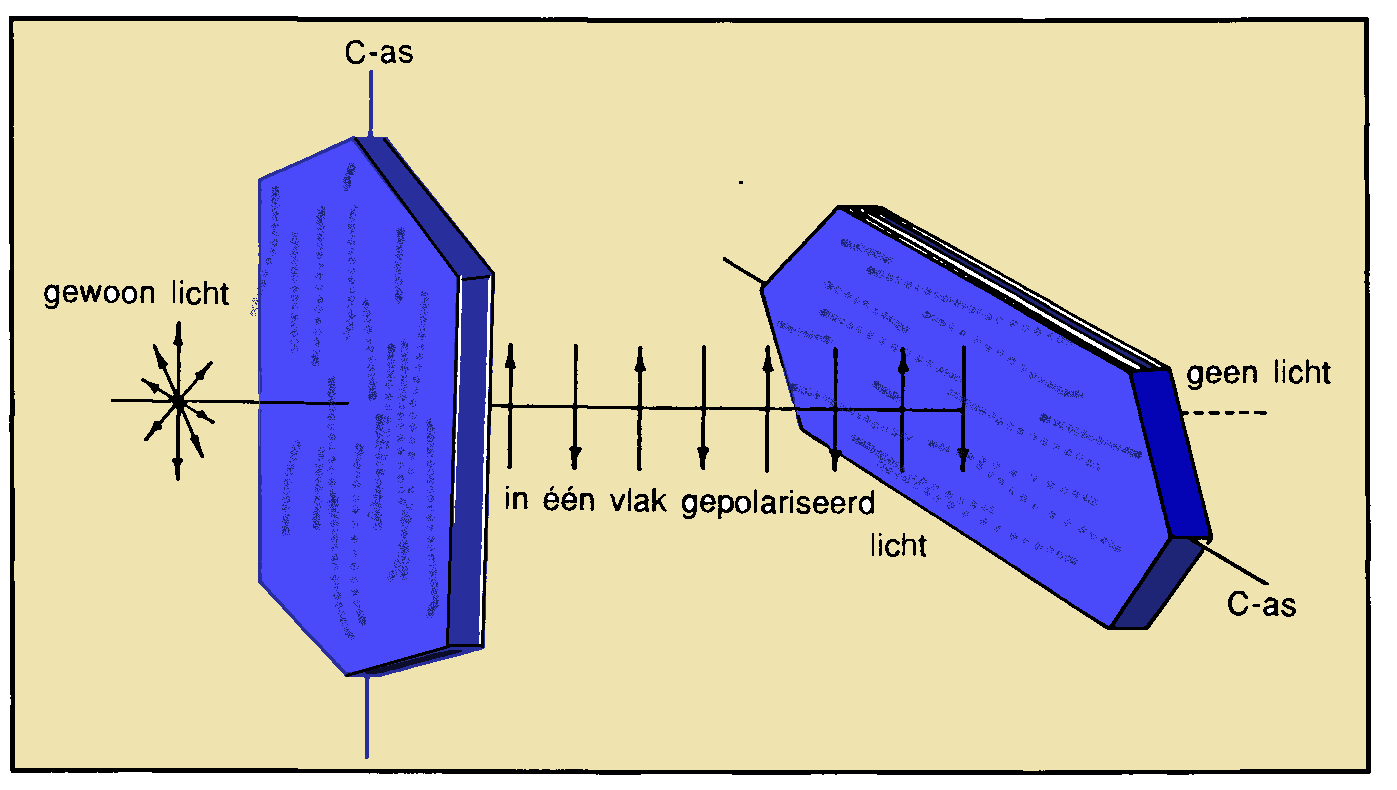
\includegraphics[width=0.5\textwidth]{./img/toermalijn.png}
\captionof{figure}{Een toermalijnkristal maakt van een ongepolariseerde lichtbundel een gepolariseerde bundel waarbij de helft van de straling wordt tegengehouden. Het tweede kristal blokkeert alle gepolariseerde straling. 
\label{fig:toermalijn}
}
\end{center}

Eigenlijk is de term filter niet helemaal juist. Een polarisatiefilter houdt inderdaad de helft van het licht tegen maar de andere helft krijgt dezelfde polarisatierichting als die van het filter. 
Malus had niet de beschikking over polarisatiefilters maar ontdekte toch de wet die naar hem genoemd is. In figuur~\ref{fig:polarisatiespaat} is die wet in beeld gebracht.

\begin{center}
\leavevmode
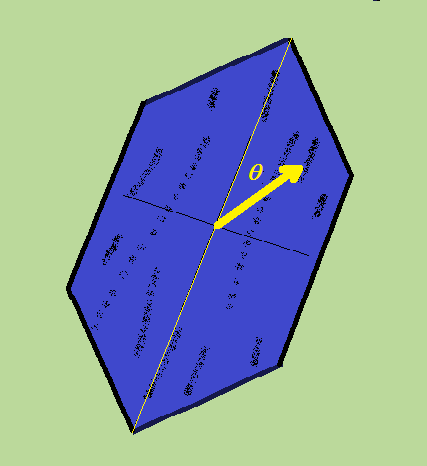
\includegraphics[width=0.5\textwidth]{./img/malus.png}
\captionof{figure}{Als een bundel gepolariseerd licht op een polarisator valt met een hoek $\theta$ tussen de polarisatierichtingen dan zal het doorgelaten licht de polarisatierichting krijgen van het filter en de intensiteit van het doorgelaten licht zal een fractie $\cos^2\theta$ zijn van het opvallende licht. (Wet van Malus) 
\label {fig:malus}
}
\end{center}

Volgens de wet van Malus geldt dat de intensiteit van de doorgelaten lichtbundel gelijk zou moeten zijn aan:
$$I=I_0 \cos^2\theta$$

Hierin is $I_0$ de intensiteit van het opvallende licht en I de intensiteit van het doorgelaten licht. De intensiteit wordt daarbij in verband gebracht met stralingsenergie en dus gemeten in \si{\watt\per\meter\squared}. Maar in de tijd van Malus was Joule nog niet geboren en de energie-eenheden bestonden nog niet. 
Dat de filters inderdaad meer doen dan filteren wordt onmiddellijk duidelijk door een derde filter tussen de beide filters van figuur~\ref{fig:toermalijn} in te schuiven. Het blijkt dat, afhankelijk van de stand van het derde filter, er weer licht door de barri\`ere komt. Het is zelfs nog erger. Door heel veel filters achter elkaar te plaatsen is het mogelijk het polarisatievlak te draaien zonder dat er licht verloren gaat! 

Nog een verrassend experiment is te zien in figuur~\ref{fig:polarisatiespaat}.

\begin{center}
\leavevmode
\includegraphics[width=0.5\textwidth]{./img/polarisatiespaat.png}
\captionof{figure}{Ongepolariseerd licht dat op een polarisatiefilter valt, laat de helft van de fotonen door die allemaal de polarisatierichting meekrijgen van het filter. Als deze fotonen op een kristal IJslandspaat vallen worden ze verdeeld over twee bundels met tegengestelde polarisatie. 
\label {fig:polarisatiespaat}
}
\end{center}

Ongepolariseerd licht kan met hulp van een polarisatiefilter omgezet worden in licht met \'e\'en polarisatierichting. Maar dat licht met \'e\'en polarisatierichting kan weer worden omgezet in twee bundels met tegengestelde polarisatierichtingen met behulp van een kristal IJslandspaat. Deze polarisatieverschijnselen worden onderzocht in de derde experimentenreeks.
\begin{experiment}{polarisatie}
polarisatie van licht
\end{experiment}

\section{Interferentie van elektromagnetische golven}
Radio, TV, smartphone en magnetron maken gebruik van elektromagnetische golven.
Het bestaan van deze golven is in 1873 door de Schotse natuur- en wiskundige James Clerk Maxwell (1831-1879) voorspeld in zijn werk "A Treatise on Electricity and Magnetism". Hij liet zien dat een veranderend magnetisch krachtveld een veranderend elektrisch krachtveld oproept dat op zijn beurt weer een veranderend magnetisch krachtveld oproept en zo verder. De voortplantingssnelheid van de golven bleek \SI{3.0E8}{\meter\per\second} in vacu\"um te zijn, precies de snelheid van het licht. Op grond hiervan nam Maxwell aan dat ook het licht een elektromagnetisch golfverschijnsel is. In 1888 slaagde Heinrich Hertz er in om elektromagnetische golven te produceren met elektrische vonken. 

\begin{center}
\leavevmode
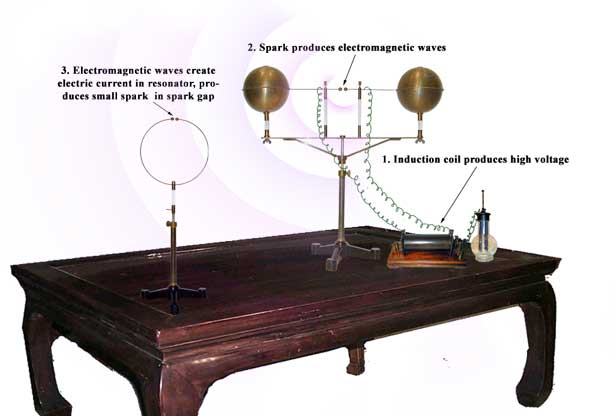
\includegraphics[width=0.5\textwidth]{./img/hertztafel.png}
\captionof{figure}{De opstelling waarmee Heinrich Hertz in 1888 de elektromagnetische golven aantoonde die Maxwell had voorspeld. Vonken, geproduceerd door de vonkgenerator aan de ene kant van de tafel veroorzaakten vonken in de trillingskring aan de andere kant van de tafel.
\label {fig:hertztafel}
}
\end{center}

In het boek "Showdefysica2" dat ongetwijfeld op school aanwezig is, staat een interferentie-experiment beschreven met een magnetron. Een magnetron produceert ook elektromagnetische golven. In de gesloten magnetron ontstaat een staande elektromagnetische golf. In figuur~\ref{fig:magnetron} is een magnetron te zien.

\begin{center}
\leavevmode
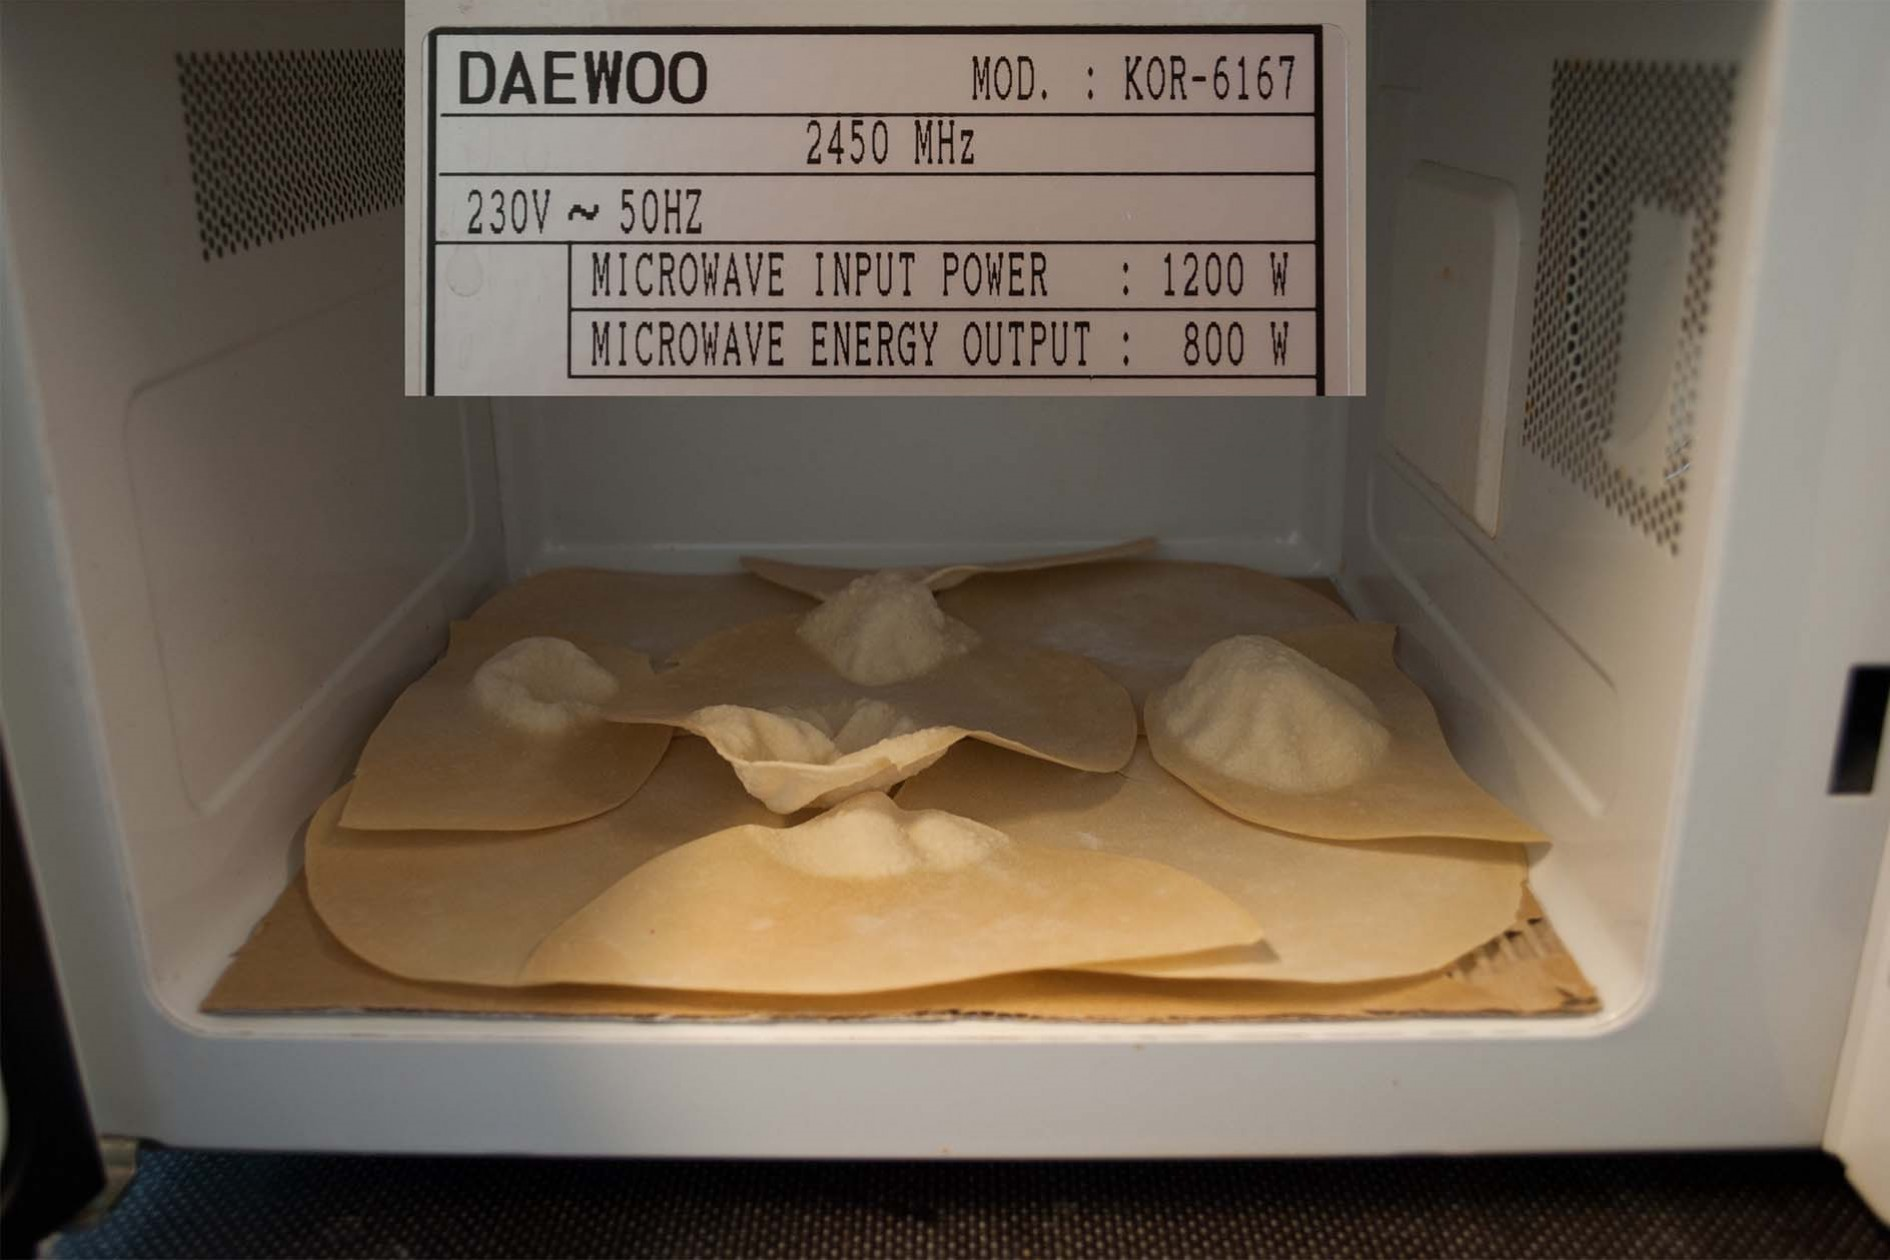
\includegraphics[width=0.5\textwidth]{./img/magnetron.png}
\captionof{figure}{Een magnetron ontstaat een staande elektromagnetische golf. In de buiken is de opwarming het sterkst. In de knopen doven de elektromagnetische golven elkaar uit. Elke magnetron heeft daarom ook een draaien schijf nodig voor de gelijkmatige opwarming.
\label {fig:magnetron}
}
\end{center}

Met behulp van speciaal voor het onderwijs ontwikkelde 3cm-golfapparatuur kunnen allerlei experimenten worden uitgevoerd. Ook een interferentie-experiment zoals dat hierboven beschreven bij geluid is mogelijk. In plaats van twee speakers zijn de golfbronnen nu twee spleten waar een zender voor is gezet. 
Het blijkt dat er ook interferentie ontstaat bij \'e\'en spleet. Zie figuur~\ref{fig:microgolf}.

\begin{center}
\leavevmode
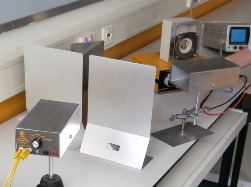
\includegraphics[width=0.5\textwidth]{./img/microgolf.png}
\captionof{figure}{Interferentie bij \'e\'en spleet.
\label {fig:microgolf}
}
\end{center}

\begin{experiment}{3~centimeter}interferentie bij 3-cm-golven met \'e\'en zender en \'e\'en ontvanger.
\end{experiment}
\hrefqr{https://www.physicsexperiments.org/index.php/experiments/trillingen-frequentie/3cm-magnetische-golven}{Uitleg hier}.


\section{De geboorte van de quantumfysica}
Mede door het werk van James Clerk Maxwell was er aan het eind van de 19e eeuw geen natuurkundige meer te vinden die nog geloofde dat licht bestond uit deeltjes. Het grote debat over de aard van het licht was voorbij. Het pleit was beslecht in het voordeel van de golftheorie van Huygens. Nieuwe vormen van elektromagnetische straling werden ontdekt, zoals de straling die Konrad R\"ontgen had gevonden die dwars door spierweefsel kon schijnen en de botten in een lichaam zichtbaar kon maken. Nieuwe toepassingen werden mogelijk door het werk van Guielmo Marconi die het fundament legde voor de ontwikkeling van radio en telegrafie. Allemaal gevolgen van de ontdekking van het elektromagnetische spectrum. Aan het eind van de 19e eeuw werd ook onderzocht hoe met de golftheorie kon worden verklaard hoe de energie verdeeld is over de stralingsgolven die worden uitgezonden door een object met een bepaalde temperatuur. Een warm voorwerp straalt warmte uit in de vorm van infraroodstraling. Slangen maken daarvan gebruik om hun prooi te vinden in een ruimte waarin geen licht is. Maar als de temperatuur van een ijzeren staaf maar voldoende oploopt gaat hij ook licht uitzenden. En de bbq in figuur~\ref{fig:temperatuurstraling} maakt onmiddellijk duidelijk dat roodgloeiend minder heet is dan geel.

\begin{center}
\leavevmode
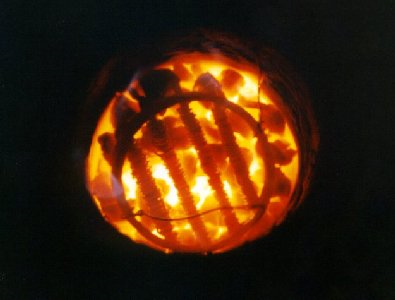
\includegraphics[width=0.5\textwidth]{./img/temperatuurstraling.png}
\captionof{figure}{Temperatuurstraling. Zowel roodgloeiende als withete plekken zijn zichtbar. Maar ook de zwarte plekken zenden straling uit. Dat is dan voornamelijk infrarode straling.
\label {fig:temperatuurstraling}
}
\end{center}

In 1900 probeerden Rayleigh en Jeans een theorie op te stellen met behulp van de golftheorie voor de verdeling van energie over de golflengten. Voor de grote golflengten lukte dat uitstekend maar voor de kleinere golflengten ging het catastrofaal mis. De discrepantie tussen theorie en experiment is bekend komen te staan als de UV-catastrofe.
In figuur~\ref{fig:catastrophe} is deze discrepantie in beeld gebracht.

\begin{center}
\leavevmode
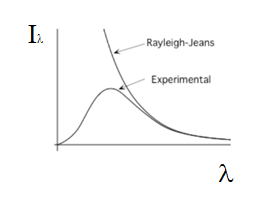
\includegraphics[width=0.5\textwidth]{./img/catastrophe.png}
\captionof{figure}{Rayleigh en Jeans vonden in 1900 een formule voor de spectrale intensiteit van temperatuurstraling. Voor grote golflengtes was het verband goed. Voor korte golflengtes was er een catastrofale afwijking tussen theorie en experiment.
\label {fig:catastrophe}
}
\end{center}

Nog datzelfde jaar kwam Max Planck (1858-19470 ) met een oplossing. Hij nam aan dat de energie was gequantiseerd. Een stralend lichaam zou zijn energie afgeven in pakketjes waarvoor gold:

$$E=hf$$

Hierin is $f$ de frequentie van het uitgezonden licht en $h$ is de zogenaamde constante van Planck. Er geldt: h = \SI{6.62607015e-34}{\joule\second}
Met deze kunstmatige ingreep kreeg Planck een perfecte overeenstemming tussen theorie en experiment. Later gaf hij toe dat de kunstgreep een soort wanhoopsdaad was. Hij is de rest van zijn leven bezig geweest om zijn quantumhypothese weer ongedaan te maken.
Nog meer problemen \ldots
Bovenop de problemen waarmee de inmiddels traditionele elektromagnetische golftheorie te kampen had kwam nog een nieuw onverklaarbaar fenomeen boven water. Dit verschijnsel staat bekend als het foto-elektrisch effect.

Als een metalen oppervlak wordt beschenen met licht komen er elektronen vrij. Dit verschijnsel werd voor het eerst ontdekt door Heinrich Hertz in 1887 toen hij onderzoek deed naar elektromagnetische golven. 

\begin{center}
\leavevmode
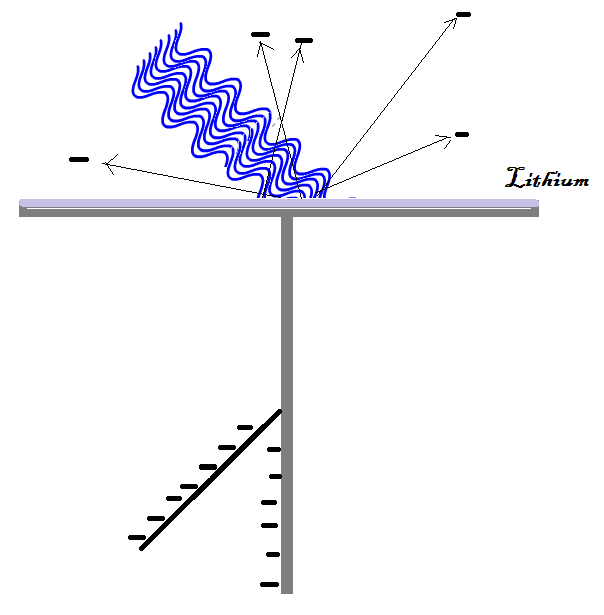
\includegraphics[width=0.5\textwidth]{./img/electroscoop.png}
\captionof{figure}{Een elektroscoop is negatief geladen en daardoor is er een uitslag te zien. Bij blauw licht neemt de uitslag af. Bij rood licht niet. Ook niet als je een felle laser gebruikt.
Einstein gaf de verklaring: lichtenergie wordt in quanten afgegeven. De blauwe fotonen hebben genoeg energie om een elektron vrij te maken maar de rode niet.
\label {fig:electroscoop}
}
\end{center}

Elektronen zijn natuurlijk gebonden aan atomen dus dan is er energie nodig om ze los te maken uit het metaal. De intensiteit van het opvallende licht moet dus wel invloed hebben op het aantal losgemaakte elektronen. Maar tot verbijstering van de toenmalige natuurkundige gemeenschap had ook de frequentie en dus de kleur van het opvallende licht invloed op de hoeveelheid elektronen die door het licht werden vrijgemaakt. Bij elk metaal was er zelfs sprake van een karakteristieke drempelfrequentie. Beneden deze waarde werden er helemaal geen elektronen vrij gemaakt. Als Lithium werd beschenen met blauw licht (hoge frequentie dus korte golflengte) kwamen er elektronen vrij maar als het werd beschenen met rood licht (lagere frequentie, langere golven) niet. Zelfs niet als de intensiteit van het opvallende licht enorm werd opgevoerd. De natuurkundigen van die tijd hadden geen enkel idee hoe dit kon worden verklaard. Uiteindelijk was er een Duitse jongen van 25 jaar voor nodig om de knuppel in het hoenderhok te gooien.

\section{Quantumrevolutie}
Iedereen kent Albert Einstein (1879-1955). In 1905 is hij 25 jaar oud en produceert dan drie publicaties die elk voor zich een Nobelprijs zouden rechtvaardigen. Maar hij kreeg hem uiteindelijk voor zijn verklaring van het foto-elektrisch effect. En de verklaring die Einstein gaf was bizar. Wat hij voorstelde kwam er op neer dat het debat tussen Newton en Huygens dat na eeuwen van dispuut in het voordeel van Huygens was uitgevallen toch weer moest worden opengebroken. Einstein maakte gebruik van het postulaat dat een paar jaar daarvoor door Max Planck was geformuleerd. De verklaring van Einstein voor het foto-elektrisch effect kwam er op neer dat de hypothese van Planck niet zomaar een rekentechnische vinding was. Een elektron kon alleen maar worden losgemaakt door \'e\'en zo'n lichtpakketje maar dan moest dat wel genoeg energie hebben. Rood licht kon daarom nooit voor emissie van elektronen uit Lithium zorgen omdat de energie van de stralingsquanten eenvoudig niet groot genoeg was om een elektron los te maken. 
De energiepakketjes van Planck zijn in de theorie van Einstein echte deeltjes geworden. We noemen ze fotonen.
Gezien de sleutelrol die het foto-elektrisch effect speelt in de quantumrevolutie is het goed om er proefondervindelijk ervaring mee op te doen.

\begin{experiment}{het foto-elektrisch effect}
FEE
\end{experiment}



\section{Nieuw bewijs: het Compton-effect}
Wie met een sterke claim komt heeft sterke bewijslast nodig. Niet iedereen ging akkoord met de verklaring van Einstein. In 1923 kwam er een onafhankelijke waarneming van een ander verschijnsel dat een sterke ondersteuning vormde voor de opvatting dat straling ook een deeltjeskarakter had. Waarneming en verklaring waren afkomstig van een Amerikaan Arthur Holly Compton (1892-1962). Wat Compton ontdekte was dat wanneer een energierijk r\"ontgenfoton op een stilstaand elektron werd geschoten, er een botsing plaats vond waarbij elektron en foton beide in verschillende richtingen verder gingen. Bekijk figuur~\ref{fig:compton}.

\begin{center}
\leavevmode
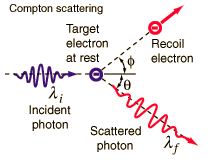
\includegraphics[width=0.5\textwidth]{./img/compton.png}
\captionof{figure}{Een foton botst tegen een elektron als was er sprake van een botsing tussen twee biljardballen. De bewegingsenergie van het elektron is afkomstig van het foton dat dus "van kleur moet verschieten" omdat zijn golflengte groter wordt.
\label {fig:compton}
}
\end{center}

Het elektron krijgt bewegingsenergie die het foton moet leveren. Aangezien de energie van een foton afhangt van zijn golflengte ($E=hf=\tfrac{hc}{\lambda}$) moet de golflengte van het foton na de botsing dus groter worden. In 1927 ontving Compton de Nobelprijs voor zijn werk.

De revolutie breidt zich uit: de hypothese van de Broglie.
Zeker na de bevindingen van Compton werd er van uitgegaan dat lichtgolven met frequentie f en golflengte $\lambda$ ook zich konden manifesteren als deeltjes met een energie E en een impuls p. De twee bruggetjes tussen golfwereld en deeltjeswereld werden gevormd door twee formules:

$$E=hf$$
$$p=\frac{h}{\lambda}$$

Het was een Franse prins die in 1924 de onvermijdelijke sprong waagde. Als golven een deeltjeskarakter konden hebben was het wellicht ook mogelijk dat deeltjes een golfkarakter konden hebben. Elektronen zouden dus ook een golflengte moeten hebben.
Het bewijs volgde drie jaar later. In 1927 toonden Davisson en Germer aan dat als elektronen werden geschoten op een kristal er achter het kristal een interferentiepatroon zichtbaar werd. In 1929 kreeg Louis de Broglie de Nobelprijs voor zijn bijdrage aan de quantumtheorie.

\section{Interpretatie van de quantumtheorie}
Door de ontwikkeling van de quantumtheorie zijn oude verschijnselen in een heel nieuw daglicht komen te staan. Dat wordt heel zichtbaar als we kijken naar het experiment met licht dat door een polarisatiefilter gaat. 
In figuur~\ref{fig:vierstanden} is een polarisatiefilter in vier verschillende standen te zien waarop steeds een fotonenstroom wordt gestuurd. Het polarisatiefilter wordt geacht ideaal te zijn. Dat houdt in dat fotonen met een polarisatierichting gelijk aan die van het filter altijd worden doorgelaten. (In werkelijkheid vindt er altijd wel wat absorptie plaats vanwege de wet van Lambert-Beer die zegt dat straling die door materiaal van een zekere dikte gaat altijd wel energie verliest.)

\begin{center}
\leavevmode
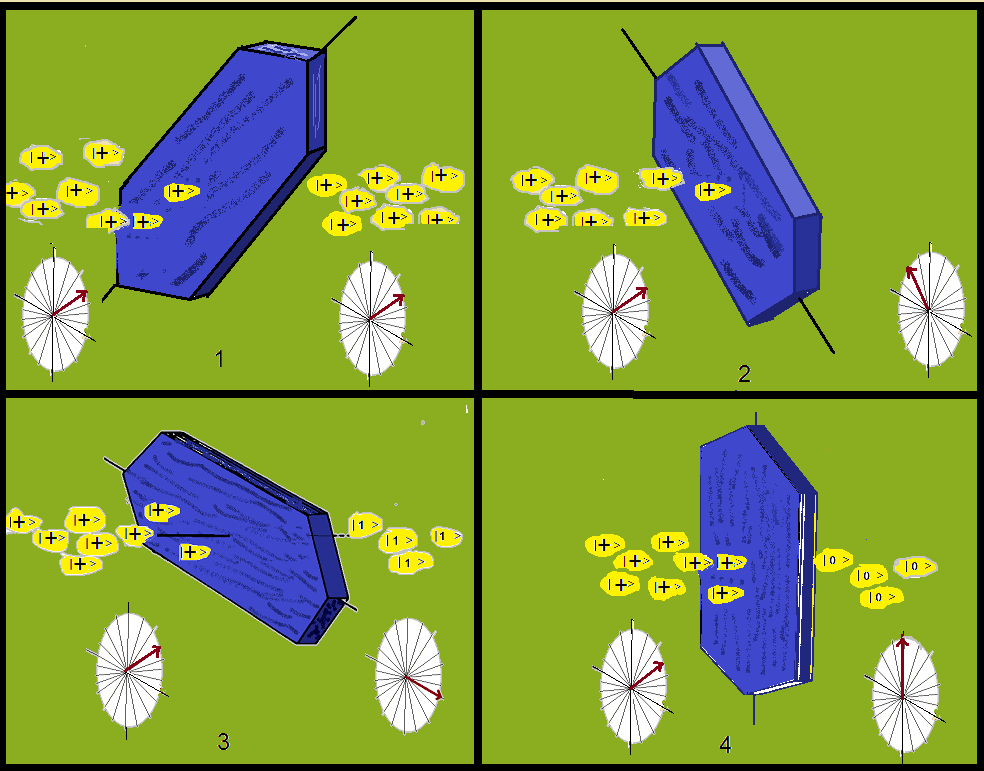
\includegraphics[width=0.5\textwidth]{./img/vierstanden.png}
\captionof{figure}{Bij afbeelding 1 komen alle fotonen door. In stand 2 wordt alles tegengehouden. In stand 3 wordt de helft tegengehouden evenals in stand 4. De fotonen die wel doorkomen hebben een andere toestand gekregen.\label {fig:vierstanden}
}
\end{center}

De opvallende fotonen hebben steeds dezelfde polarisatierichting 450 vanaf de verticaal. In afbeelding 1 komt de stand van het polarisatiefilter overeen met de polarisatierichting van de opvallende fotonen. Alle fotonen worden doorgelaten. Wordt het filter 900 gedraaid dan wordt er niets meer doorgelaten. Maar in andere standen gebeurt er iets met de fotonen. In verticale stand wordt 50% van de fotonen tegengehouden en in horizontale stand evenzo. De fotonen die wel door het filter gaan hebben een andere toestand gekregen. Hun polarisatierichting is gelijk geworden aan die van het filter. 

\section{Fotonen \'e\'en voor \'e\'en}
Hoe merkwaardig de fotonentheorie van het licht is volgt uit het feit dat hoewel de fotonen in plaatje 3 en 4 volmaakt identiek zijn en onderling in niets verschillen toch met de helft het ene gebeurt en met de andere helft het andere. Er is sprake van een zuiver toevalsproces. 
Het is in principe mogelijk om slechts \'e\'en foton op het filter af te sturen. Of het foton in plaatje 3 het filter passeert of niet is van tevoren volstrekt onvoorspelbaar. Het kansproces waarvan hier sprake is, is merkwaardig en in niets te vergelijken met kansprocessen in de klassieke wereld. Neem bijvoorbeeld het opwerpen van een munt die neerkomt op de kopzijde. Een film die van het proces gemaakt wordt en die beeldje voor beeldje wordt geanalyseerd laat zien dat de toestand van de munt op ieder beeld volledig met de natuurwetten kan worden voorspeld aan de hand van het beeld dat er aan voorafgaat. Twee worpen met verschillende uitkomst moeten altijd verschillend zijn geweest. Dat het opwerpen van een munt toch wordt beschouwd als een kansproces heeft te maken met het feit dat het te moeilijk is om een voorspelling te doen. Eigenlijk komen in de klassieke wereld alleen maar pseudo-kansprocessen voor.
In zijn "\textit{Essai philosophique sur les probabilit\'es}" (1814) schrijft de grote wiskundige en filsoof Laplace dat een superieure geest met kennis van alle posities en snelheden van alle deeltjes toekomst en verleden zou kennen. Omdat de toekomst dus volledig vastligt in deze gedachtegang noemt men dit wereldbeeld deterministisch. 
Laplace was echter onbekend met de quantumwereld. De fotonen die in figuur~\ref{fig:vierstanden} het polarisatiefilter passeren verschillen in niets van de fotonen die door het filter worden tegengehouden. Hier is sprake van een zuiver toevalsproces. Tegenwoordig is het mogelijk om individuele fotonen uit te zenden en ook te detecteren. Maar meting aan \'e\'en foton levert dus geen echte informatie op. De metingen moeten voor heel veel fotonen worden gedaan en dat levert pas de informatie over de toestand van de fotonen op. De wereld is in essentie statistisch.
Van zulke quantumfysische toevalsprocessen zijn meer voorbeelden te geven. Het meest bekende voorbeeld is wel dat van radioactief verval. 
}%\tagged{eruit%\fi----

